\documentclass{article}
\usepackage{polski}
\usepackage[utf8]{inputenc}
\usepackage{indentfirst}
\usepackage{fancyhdr}
\usepackage{fancyvrb}
\usepackage{natbib}
\usepackage{lastpage}
\usepackage{graphicx}

\pagestyle{fancy}
\lhead{Spis treści}
\rhead{A. Kasprzak}
\cfoot{Strona \thepage \hspace{1pt} z \pageref{LastPage}}
\begin{document}

\font\myfont=cmr12 at 28pt
\title{\myfont Corona taxi $-$ Specyfikacja funkcjonalna, projekt grupowy}
\author{ \Huge Arkadiusz Kasprzak\\[8pt] \Huge Jakub Komorowski\\[8pt] \Huge Marcin Kowalczyk }
\date{\huge 01.12.2020.}
\maketitle

\thispagestyle{empty}
\newpage

\begin{frame}{}
    \tableofcontents
\end{frame}

\lhead{Specyfikacja funkcjonalna}
\rhead{A. Kasprzak, J. Komorowski, M. Kowalczyk}
\newpage

\section{Opis ogólny, założenia projektowe}
    
    Głównym celem projektu jest stworzenie programu o nazwie "Corona Taxi", mającego pomóc Służbie Ochrony Zdrowia. Będzie to możliwe, dzięki optymalizacji ruchu Karetek Pogotowia - odbioru oraz transportu Pacjenta do najbliższego (w linii prostej) Ośrodka Medycznego. W przypadku braku wolnych miejsc w Ośrodku medycznym, pacjent zostanie przetransportowany do kolejnego, najbliższego Ośrodka Medycznego (jednakże w tym przypadku, odległość do kolejnych placówek jest mierzona po drogach). Informacje o:
    
    \begin{itemize}
        \item położeniu Pacjentów, 
        \item położeniu Ośrodków Medycznych,
        \item położeniu Obiektów - neutralnych elementów, będących częścią kraju,
        \item drogach - połączeniach między Ośrodkami Medycznymi,
        \item liczbie wszystkich łóżek w danym Ośrodku Medycznym,
        \item liczbie wolnych łóżek w danym Ośrodku Medycznym,
    \end{itemize}
    będą dostarczane do programu przez Dyspozytora Pogotowia.
    Ograniczenia:
    
    \begin{itemize}
        \item Granice kraju będą ograniczane przez najbardziej oddalone od siebie \\punkty - jest to najmniejszy zbiór wypukły zawierający w sobie wszystkie Ośrodki Medyczne oraz Obiekty.
        \item Pacjenci znajdujący się poza granicami kraju nie będą obsługiwani.
    \end{itemize}
    Założenia:
    
    \begin{itemize}
        \item Karetka Pogotowia sama dojeżdża do miejsca pobytu Pacjenta (jej ruchem zaczynamy kierować w momencie podjęcia Pacjenta).
        \item Karetka Pogotowia może przewozić tylko jednego pacjenta na raz.
        \item W miejscach przecięcia się dróg znajdują się skrzyżowania.
        \end{itemize}
    Program będzie interaktywny, a korzystanie z niego będzie możliwe poprzez interfejs graficzny.

\section{Opis funkcjonalności}
    Program będzie realizował następujące funkcje:
    \begin{itemize}
        \item Weryfikacja poprawności otrzymanych danych z obu plików tzn. sprawdzenie czy:
            \begin{itemize}
            \item dane są odpowiednich typów.
            \item dany plik nie jest pusty.
            \item dane nie przekraczają założonych wartości.
            \end{itemize}
        \item Dostarczenie pacjentów do najbliższych, niezajętych szpitali.
        \item Zmiana prędkości odtwarzania animacji.
        \item Wyświetlanie informacji o ruchach pacjentów.
        \item Dodanie pacjenta z poziomu GUI.
    \end{itemize}

\section{Format danych i struktura folderów}

    \subsection{Struktura folderów}
        Wszystkie elementy składowe programu będą znajdowały się w odpowiednich folderach. W projekcie rozróżniamy cztery główne foldery:

        \begin{itemize}
            \item[I.] data - folder, w którym będą przechowywane dane wejściowe używane przez program.
            \item[II.] documentation - folder, w którym będzie znajdowała się cała dokumentacja projektu tzn. specyfikacja funkcjonalna i specyfikacja implementacyjna.
            \item[III.] src - główny folder programu, który będzie zawierał cały kod odpowiedzialny za działanie programu.
            \item[IV.] test - W tym folderze będą umieszczone wszystkie testy, które zostaną przeprowadzone, aby sprawdzić poprawne funkcjonowanie programu.
        \end{itemize}

    \subsection{Format danych}
        Program będzie przyjmował dwa pliki. Będą one posiadały następujące informacje:
        \begin{itemize}
            \item[I.]
            \begin{itemize}
                \item Lista szpitali zawierająca:
                    \begin{itemize}
                        \item unikalne id (liczba całkowita nieujemna)
                        \item unikalna nazwa (ciąg znaków, nie dłuższy niż 40 znaków)
                        \item współrzędne x (liczba całkowita)
                        \item współrzędne y (liczba całkowita)
                        \item liczba wszystkich łóżek (liczba całkowita nieujemna)
                        \item liczba wolnych łóżek (liczba całkowita nieujemna)
                    \end{itemize}
                \item Lista obiektów zawierająca:
                    \begin{itemize}
                        \item unikalne id (liczba całkowita nieujemna)
                        \item unikalna nazwa (ciąg znaków, nie dłuższy niż 40 znaków)
                        \item współrzędne x (liczba całkowita)
                        \item współrzędne y (liczba całkowita)
                    \end{itemize}
                \item Lista dróg między szpitalami zawierająca:
                    \begin{itemize}
                        \item unikalne id (liczba całkowita nieujemna)
                        \item id pierwszego szpitala (z wcześniej wspomnianej listy szpitali)
                        \item id drugiego szpitala (z wcześniej wspomnianej listy szpitali)
                        \item odległość między tymi szpitalami
                    \end{itemize}
                \end{itemize}
            \item[II.]
                \begin{itemize}
                    \item Lista pacjentów zawierająca:
                    \begin{itemize}
                        \item unikalne id pacjenta (liczba całkowita nieujemna)
                        \item współrzędne x (liczba całkowita)
                        \item współrzędne y (liczba całkowita)
                    \end{itemize}
                \end{itemize}
        \end{itemize}
        
    \begin{figure}[h]
    \centering
    \includegraphics[scale=0.7]{Wzór pliku ze szpitalami.png}
    \caption{Wzór pierwszego pliku.}
    \end{figure}
    
    \begin{figure}[h]
    \centering
    \includegraphics[scale=1]{Wzór pliku z pacjentami.png}
    \caption{Wzór drugiego pliku.}
    \end{figure}
    
\section{Opis graficznego interfejsu użytkownika}
    Graficzny interfejs użytkownika będzie znajdował się w nieskalowalnym oknie, wypełniającym cały ekran. Interfejs zostanie podzielony na dwie główne części (Patrz rys. 2): część w której wyświetli się mapa szpitali, obiektów i pacjentów, oraz część obsługową, umożliwiającą użytkownikowi: wprowadzenie nazw plików z danymi, ustawienie prędkości wyświetlania kolejnych przejazdów pacjentów, oraz sekcję wyświetlającą przejazdy kolejnych pacjentów między szpitalami.
    
    \begin{center}
        
\includegraphics[scale = 0.05]{Ikonka.jpg}
        \textit{\\Rys. 3. Ikona programu\\}
        
        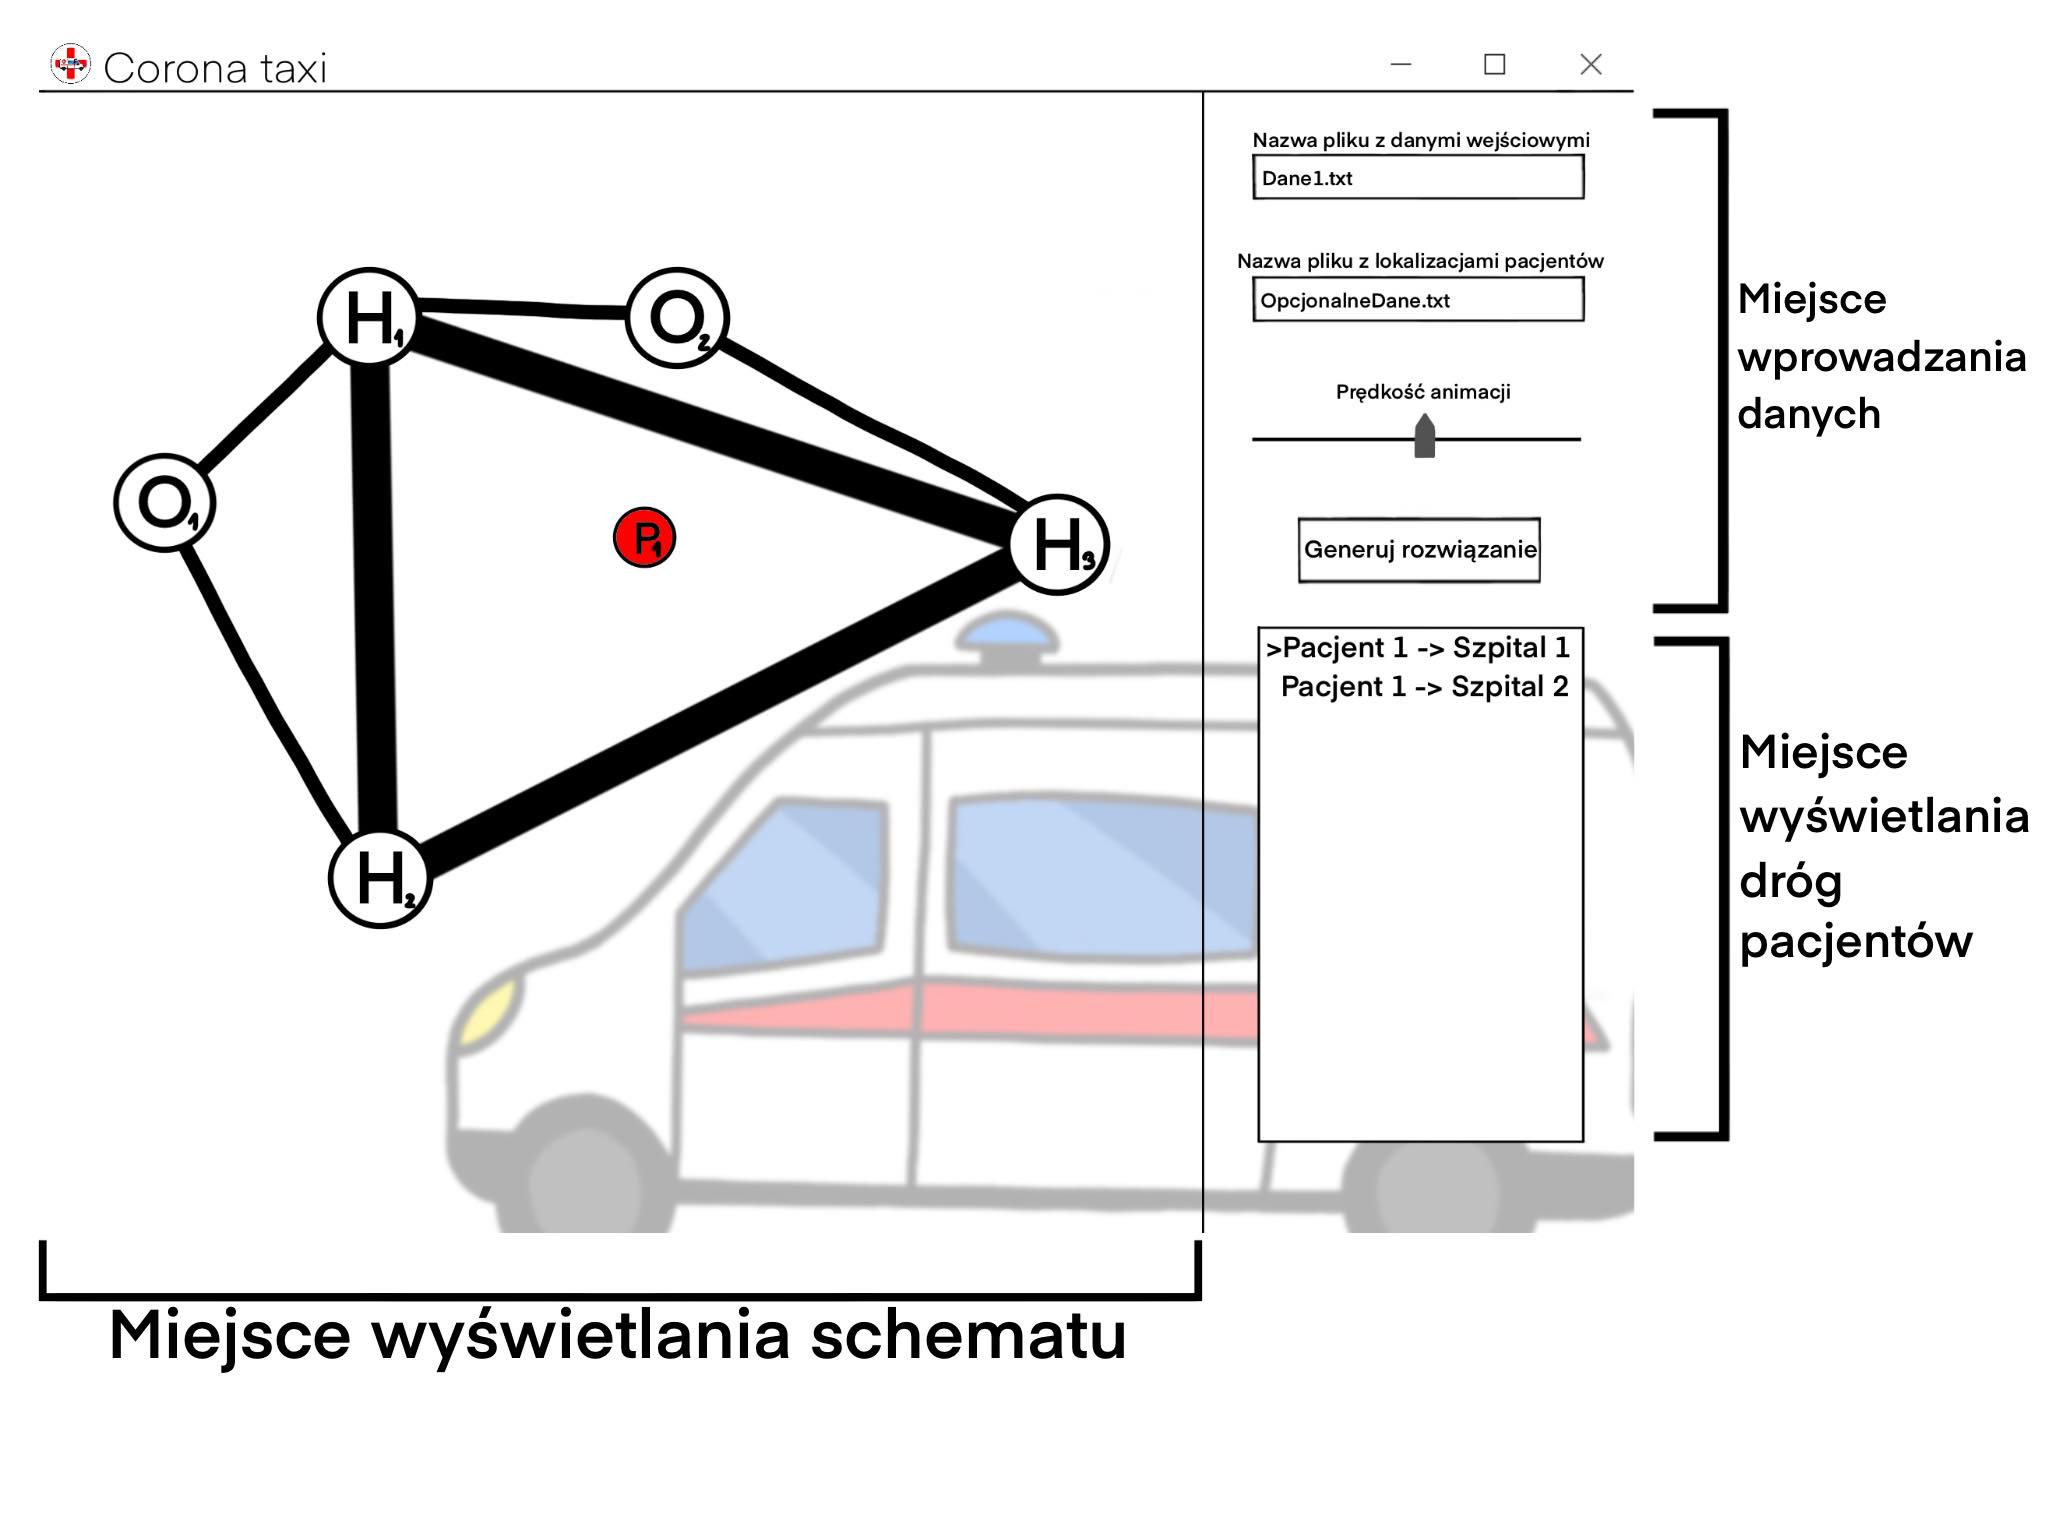
\includegraphics[scale = 0.18]{SchematGUI.jpg}
        \textit{\\Rys. 4. Wizualizacja GUI programu, z opisem poszczególnych części\\}
    \end{center}


\section{Potencjalne komunikaty o błędach}
    W przypadku wprowadzenia nieprawidłowych danych wejściowych, program poinformuje o tym użytkownika poprzez następujące komunikaty:
    \begin{itemize}
        \item \textbf{Błędny format pliku!} – komunikat wyświetlany w przypadku, gdy dostarczony plik jest w nieodpowiednim formacie.

        \item \textbf{Błędna struktura pliku!} – komunikat wyświetlany w przypadku, gdy
        w pliku z danymi wejściowymi brakuje któregoś nagłówka, lub gdy liczba
        kresek pionowych „$|$” jest nieprawidłowa.

        \item \textbf{Niepoprawne dane!} – komunikat wyświetlany w przypadku, gdy któryś
        parametr będzie zawierał niepoprawne dane, np. w miejscu parametru id
        znajdzie się litera.

        \item \textbf{Podany plik wejściowy jest pusty!} - komunikat wyświetlany w przypadku, gdy dostarczony plik nie ma zawartości.
        
        \item \textbf{Dane w pliku nie mogą przekraczać następujących wartości:} - komunikat wyświetlany w przypadku, gdy dane w pliku będą zbyt duże. Po tym komunikacie zostaną wypisane maksymalne wartości poszczególnych typów danych przyjmowane przez program.
    \end{itemize}

\section{Testowanie}
    Poprawne działanie programu zostanie zweryfikowane za pomocą testów jednostkowych, napisanych we frameworku TestNG. Poza tym zostaną przeprowadzone manualne testy Graficznego Interfejsu Użytkownika.

\end{document}